\section{Frequnzverhalten analoger LTI-Systeme}


\subsection{Zusammenhang Frequenzgang -- UTF}

Alle LTI-Systeme lassen sich mit einer Differntialfleichung der folgenden Form beschreiben:
$$ DGL $$

Die Laplace-Transformierte der DGL hat die Form 
$$ Laplace $$


\begin{tabular}{ll}
    $N(s)$ & Zählerpolynom \\
    $D(s)$ & Nennerpolynom 
\end{tabular}



\subsubsection{Umrechnung}

$$ \boxed{ H(j \omega) = H(s) \Big|_{s = j \omega}} = |H(j \omega)| \cdot e^{j \theta(\omega)} $$


\begin{tabular}{ll}
    $H(s)$          & Übertragungsfunktion (UTF) \\\
    $H(j \omega)$   & Frequenzgang \\
    $|H(j \omega)|$ & Amplitudengang \\
    $\theta(\omega)$& Phasengang
\end{tabular}


\subsection{Bestimmung Frequenzgang aus UTF}




\subsection{Pol- und Nulstellendiagramme}

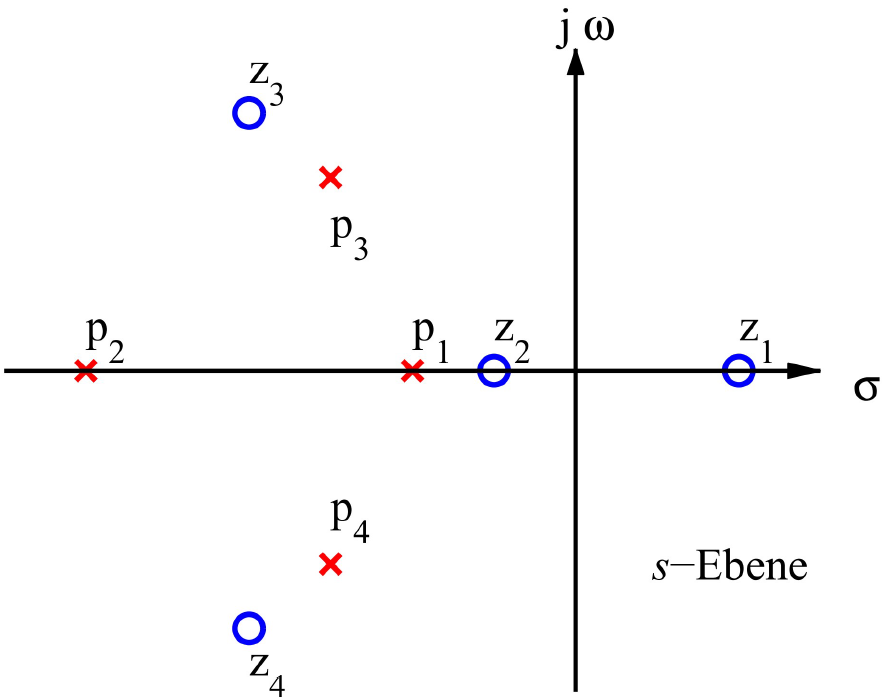
\includegraphics[width=0.6\columnwidth]{images/pol_nullstellen_diagramm.png}



\subsection{Bestimmung Frequenzgang aus Pol-/ NS der UTF}


